%
\section{Database Design}

Around the world there are a lot of different types of databases \cite{bib1}. We have chosen to use MySQL, the most popular - relational database. Relational databases are easy to understand \cite{bib2} and use. Relational databases are collections of relations, this type of organization and structuring of the dataset meets our requirements, and can be used for our project.

\subsection{Why MySQL?}

There are many different relational databases [3] and choosing the right one can be difficult. Our choice was MySQL database, because it is:

\begin{itemize}
	\item Open source database
	\item Ease to use
	\item Fast performance
	\item Reliable 
	\item Most popular open source DB in the world
	\item It is used by Yahoo!, Alcatel-Lucent, Google, Nokia, YouTube and many others
\end{itemize}

\subsection{ER Diagram}

Design of the database starts at the modeling phase. One of the most popular approaches is conceptual modeling, using entity relational diagram (ER) \cite{bib4}. Entity relational diagrams shows collections of relations in the modeling database. ER diagram makes it easy to understand the concept of the database. Another methodology to model databases is UML diagrams. Most OOP programmers are familiar with UML and this could make it easier for them to understand the modeling database. In the modeling and design phases ER diagrams was used and later it was converted to UML [Appendix B].

\begin{figure}[h]
	\centering
		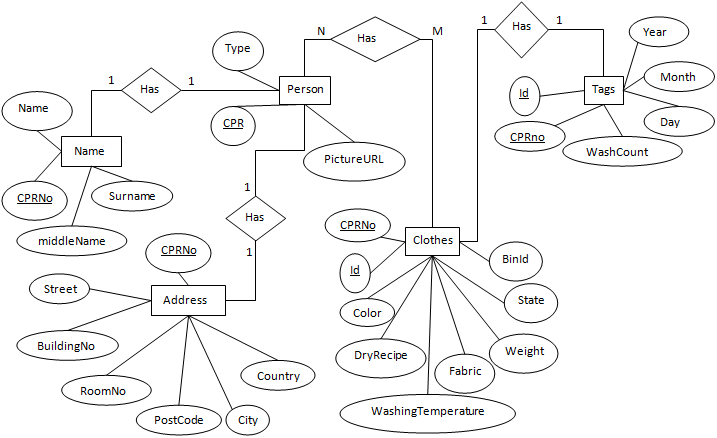
\includegraphics[scale=0.7]{erDiagramSmall}
	\caption{Laundry ER diagram}
	\label{fig:planning}
\end{figure}

\subsection{Implementation}

Before making the database tables are needed to be created and then they are moved into the database. Database tables were created by using a query language like shown in the figure \ref{fig:personAndNamesTable}. All the code was written into a text file and the text file was uploaded directly to database by using the created configurator tool.

\begin{figure}[h]
	\centering
		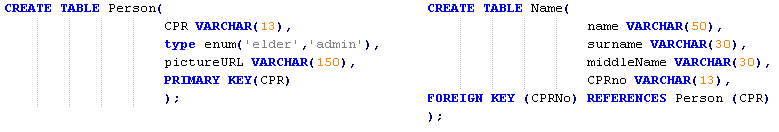
\includegraphics[scale=0.6]{personAndNamesTable}
	\caption{Person and Name tables}
	\label{fig:personAndNamesTable}
\end{figure}

The person table has three attributes: CPR, type and pictureURL and primary key for CPR. The primary key makes the table unique, without a key the table would become a weak entity type, note that it is always good to have tables with strong entity types \cite{bib4}. Foreign key also makes the table name unique. The table name has one unique reference to the person table and the person table is unique. \\ A configurator was created to make it easy to manage the database, which is able connect to database and configure by a query language or send files with configuration sentences. This makes it faster to update and change without the need of writing database code. 

\subsection{Future Work}

The usage of all tables is not optimal and/or optimized and some attributes can be unnecessary and are not used at all at present time, the space usage can be decreased. The system has not been designed with speed considerations in mind and the speed can be increased. Using strong entities instead of weak will make indexing of all the members (like hash table) possible and searching by index can improve the speed considerably.